\begin{savequote}[8cm]
\textlatin{Neque porro quisquam est qui dolorem ipsum quia dolor sit amet, consectetur, adipisci velit...}

There is no one who loves pain itself, who seeks after it and wants to have it, simply because it is pain...
  \qauthor{--- Cicero's \textit{de Finibus Bonorum et Malorum}}
\end{savequote}

\chapter{\label{ch:6-hnl}HNL} 

\minitoc


    \subsection{Heavy Neutral Leptons (HNL)}
    \subsubsection{Background}
        As a detailed review of HNL would exceed the scope of this report, only a highly simplified introduction to HNL is given here. The origin of the neutrino mass is still a mystery. 
        one intuitive solution is to extend the neutrino family to include heavy members, which mix with the existing SM neutrinos via an extended PMNS matrix and give them the small masses observed via the see-saw mechanism~\cite{Abada_2007}. As they mix the SM neutrinos, they could be produced in the intense neutrino beam in the long-baseline neutrino experiments, so the near detector of these experiments is the best place to look for HNL. The signal comes from HNL decays, some of which are distinct from SM neutrino interactions. Previously, T2K has searched for HNL~\cite{T2K:2019jwa} using the TPCs, a combined volume of about $7~\textrm{m}^3$, in ND280. As the ND280 upgrade replaces the P0D with SFGD and HATPC, a combined volume of $8~\textrm{m}^3$, which are much better trackers than the P0D, they could be used in an HNL search as well, thereby improving the overall sensitivity. 

        To perform such an HNL search, a complicated chain of simulations is required, including the generation of an HNL flux based on the SM neutrino flux, the propagation of HNL and the decay of HNL. The previous T2K search was based on a dedicated tool-set, \code{nd280HNLSim}, which was built only to search for $N\rightarrow l + \pi$ decay channels, where $l$ is a lepton. It would require a large amount of efforts to extend it to include other production and decay channels. Hence, I adapt the recently published general HNL package, \code{BeamHNL}~\cite{Plows:2022gxc}, to the T2K ND280 simulation to evaluate the sensitivity improvement brought by the upgrade.

    \subsubsection{Implementation}
        As \code{BeamHNL} aims to be a cross-experiment package, it requires a standardised flux input, the \code{dk2nu} format. Hence, I wrote the conversion program to convert the T2K flux file to a \code{dk2nu} file. Before running subsequent steps, we validate that if we feed the T2K \code{dk2nu} file to \code{BeamHNL} and set the HNL mass, $\mn$, to a small value, such as $1~\kev$, the output HNL flux should closely mimic the SM flux. The result is shown in Fig.~\ref{fig:hnl-fluxes}, which shows that the pink dash line ($\mn=1~\kev$) overlaps closely with the black solid line, which plotted directly from the T2K input flux.  
        \begin{figure}[!htb] 
            \centering 		
            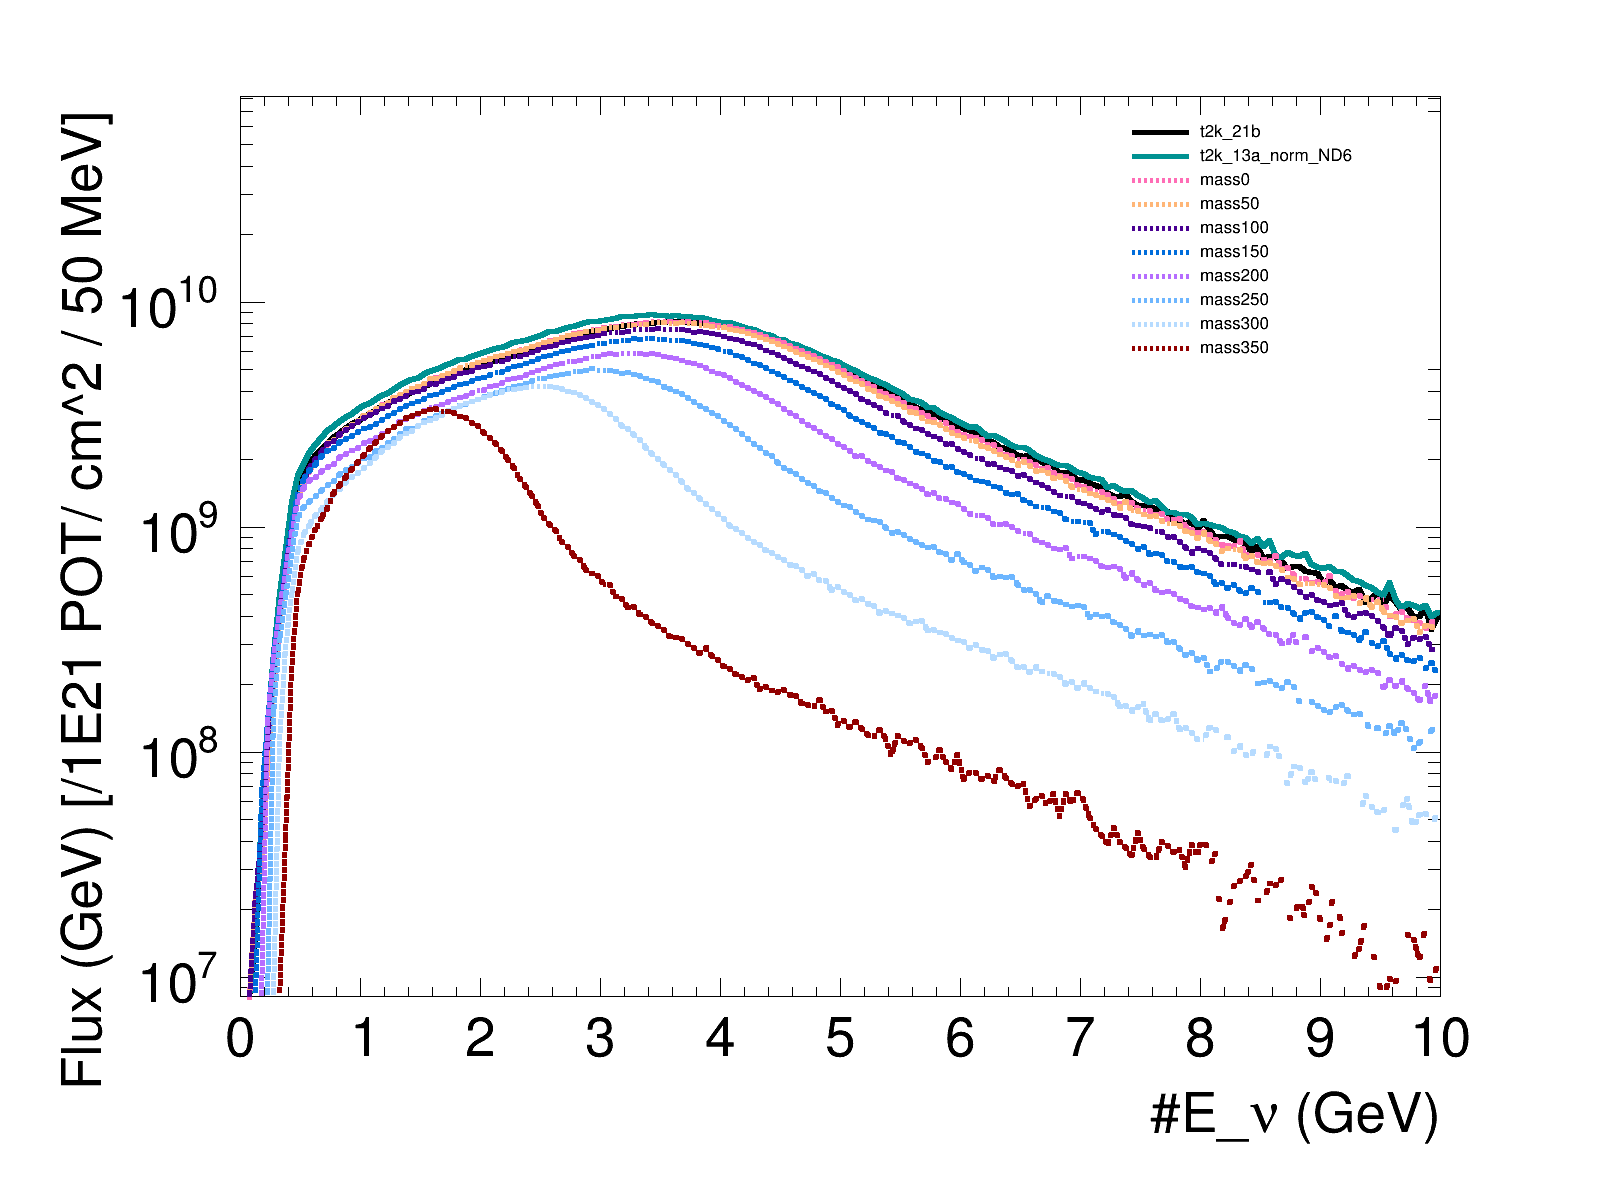
\includegraphics[width=0.45\textwidth]{fig/hnl_fluxes.png}
            \caption{\label{fig:hnl-fluxes} HNL fluxes produced by \code{BeamHNL} for different $M_N$. The solid lines are directly plotted from T2K input flux files, one with version ``13a'' and another with ``21b''. The dash lines are \code{BeamHNL} outputs for different $\mn$.} 
        \end{figure}
        After the validation, the HNL mass is then set to target values, e.g. $300~\mev$, to generate HNL events, which are then passed through the T2K simulation chain for selection development. 
        \begin{figure}[!htb] 
            \centering 		
            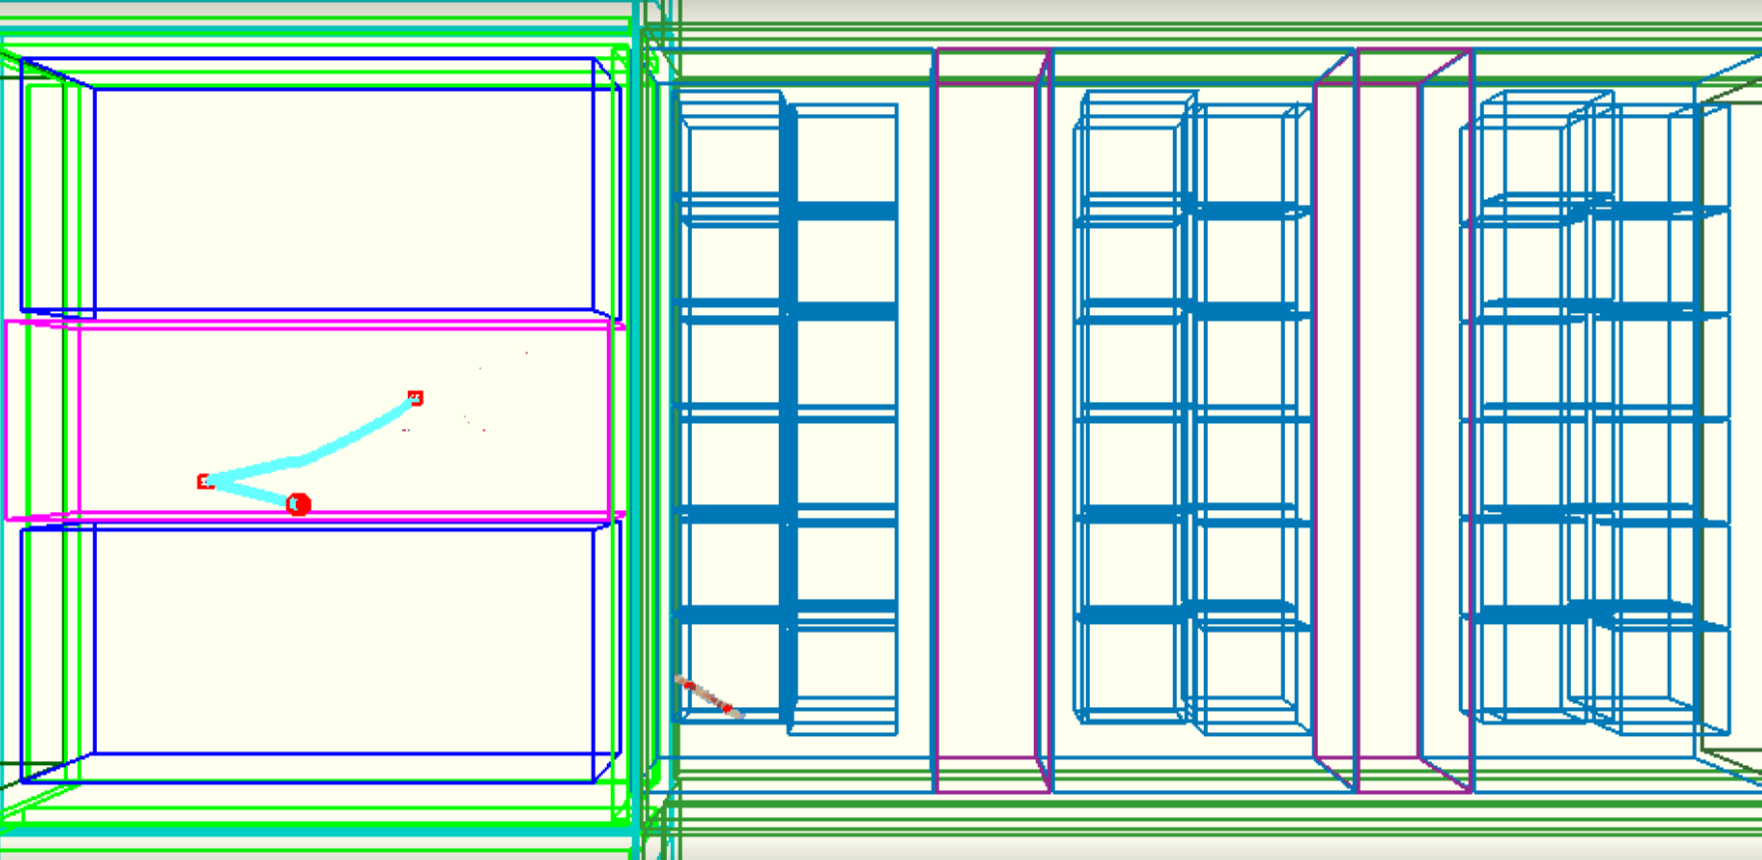
\includegraphics[width=0.45\textwidth]{fig/HNLEveDIs.png}
            \caption{\label{fig:hnl-evedis} A $N\rightarrow\mu+\pi$ event display in the upgraded ND280.} 
        \end{figure}

        It is natural to begin with the development of selecting the same signal channel as the previous T2K search to cross-validate before extending to more channels. Hence, I first developed the selection for the $N\rightarrow\mu+\pi$ channel. The steps are as follows:

        \begin{enumerate}
            \item \textbf{Basic T2K Event Quality Steps} 
            \item \textbf{Find SFGD Primary Vertex} 
            \item \textbf{No. of primary tracks cut} 
            \item \textbf{Escaping muon cut} 
            \item \textbf{One Trackless pion cut}
            \item \textbf{Kink cut}
            \item \textbf{$\mu$-$\pi$ angle and invariant cut}
            \item \textbf{$\mu$-$\pi$ $\dpt$ cut}
        \end{enumerate}

        \textbf{Basic T2K Event Quality Steps} - A quality check ensures the event contains at least $1$ reconstructed track.

        \textbf{Find SFGD Primary Vertex} - Find a primary vertex in SFGD. 
        As the primary vertex for an HNL event does not necessarily include a muon like in the $\numucc$ selection, a primary vertex should be identified independently from finding a primary muon. 
        All vertices are looped through to record the number of tracks connected to each vertex, $n_{ptrk}$ and the length of the longest track connected to each vertex, $L_{max}$. 
        The vertex with the longest $L_{max}$ is selected as the primary vertex. 
        If there is more than one such vertex, the vertex with the largest $n_{trk}$ is selected. 
        If there is still more than such one vertex, the vertex with the earliest time is selected.

        \textbf{No. of primary tracks cut} - As the target channel is $N\rightarrow\mu+\pi$, there should at most be two primary tracks. Hence, events with $n_{ptrk}>2$ are rejected.

        \textbf{Escaping muon cut} - A standard step to identify a muon escaping SFGD.

        \textbf{One Trackless pion cut} and \textbf{Kink cut} - They are the same as those in $\numuccopi$-Trackless, selecting a primary pion that has not undergone secondary interaction to ensure accurate reconstruction of its kinematics.

        \textbf{$\mu$-$\pi$ angle and invariant mass cut} - These are kinematic cuts exploiting the fact that the SM events with $1$ muon and $1$ pion are mostly resonance events that has one more proton than the HNL decay. 
        Due to the additional proton, the opening angle between the $\mu$ track and the $\pi$ track, $\tmupi$, can have large variations while that of an HNL decay would be more collimated. 
        Similarly, the invariant mass of the $\mu$-$\pi$ system, $\mmupi=(\pmu+\ppi)^2$ would have a larger range compared to the HNL, which centres around the input value, $300~\mev$ as shown in Fig.~\ref{fig:hnl-mmupi}.
        The stark contrast is apparent in Fig.~\ref{fig:mmupi-mupiang}, and to preserve the most number of HNL events, the specific cuts are: $30\degree<\tmupi<90\degree$ and $270~\mev<\mmupi<320~\mev$. 
        \begin{figure}[!htb]
           \centering
           \begin{subfigure}{0.45\textwidth}
                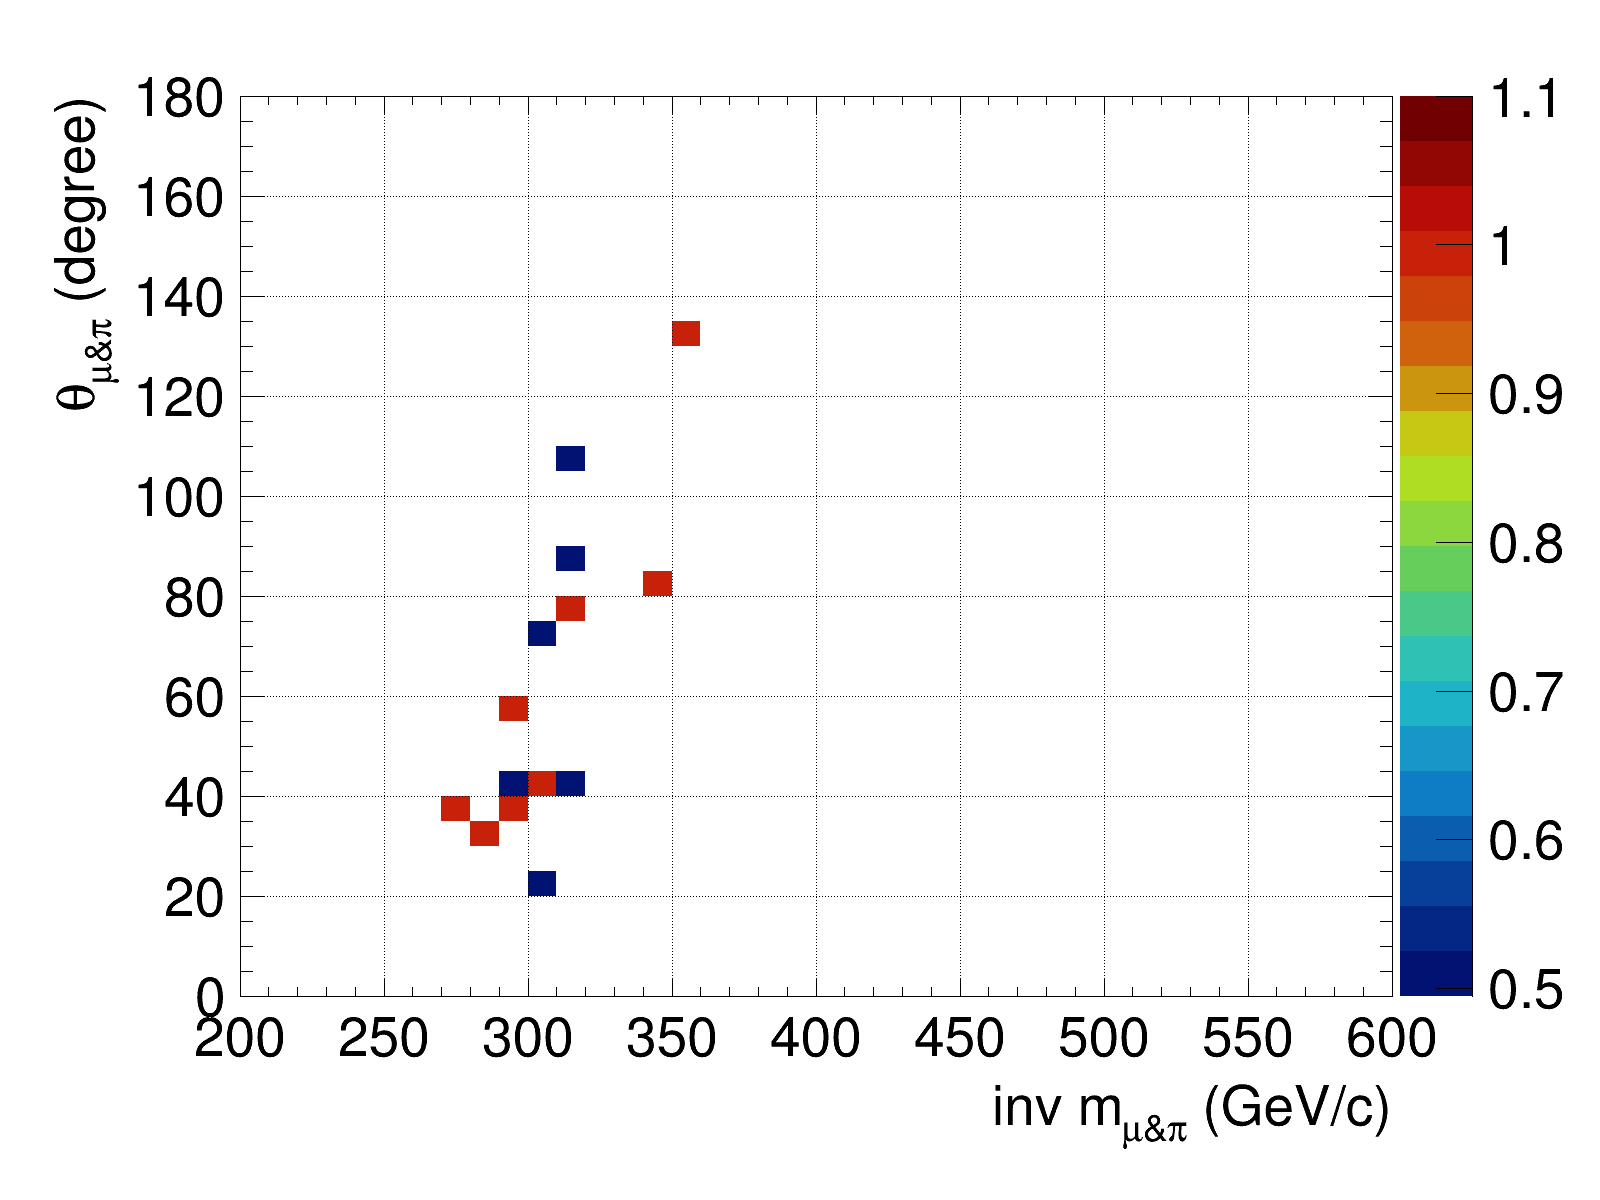
\includegraphics[width=\textwidth]{fig/hnl_sfgmu_mpinvm_colnor_vs_mpang_hist2d_al9_300.png}
                \caption{HNL.}
                \label{fig:hnl-mmupi}
           \end{subfigure}
           \begin{subfigure}{0.45\textwidth}
                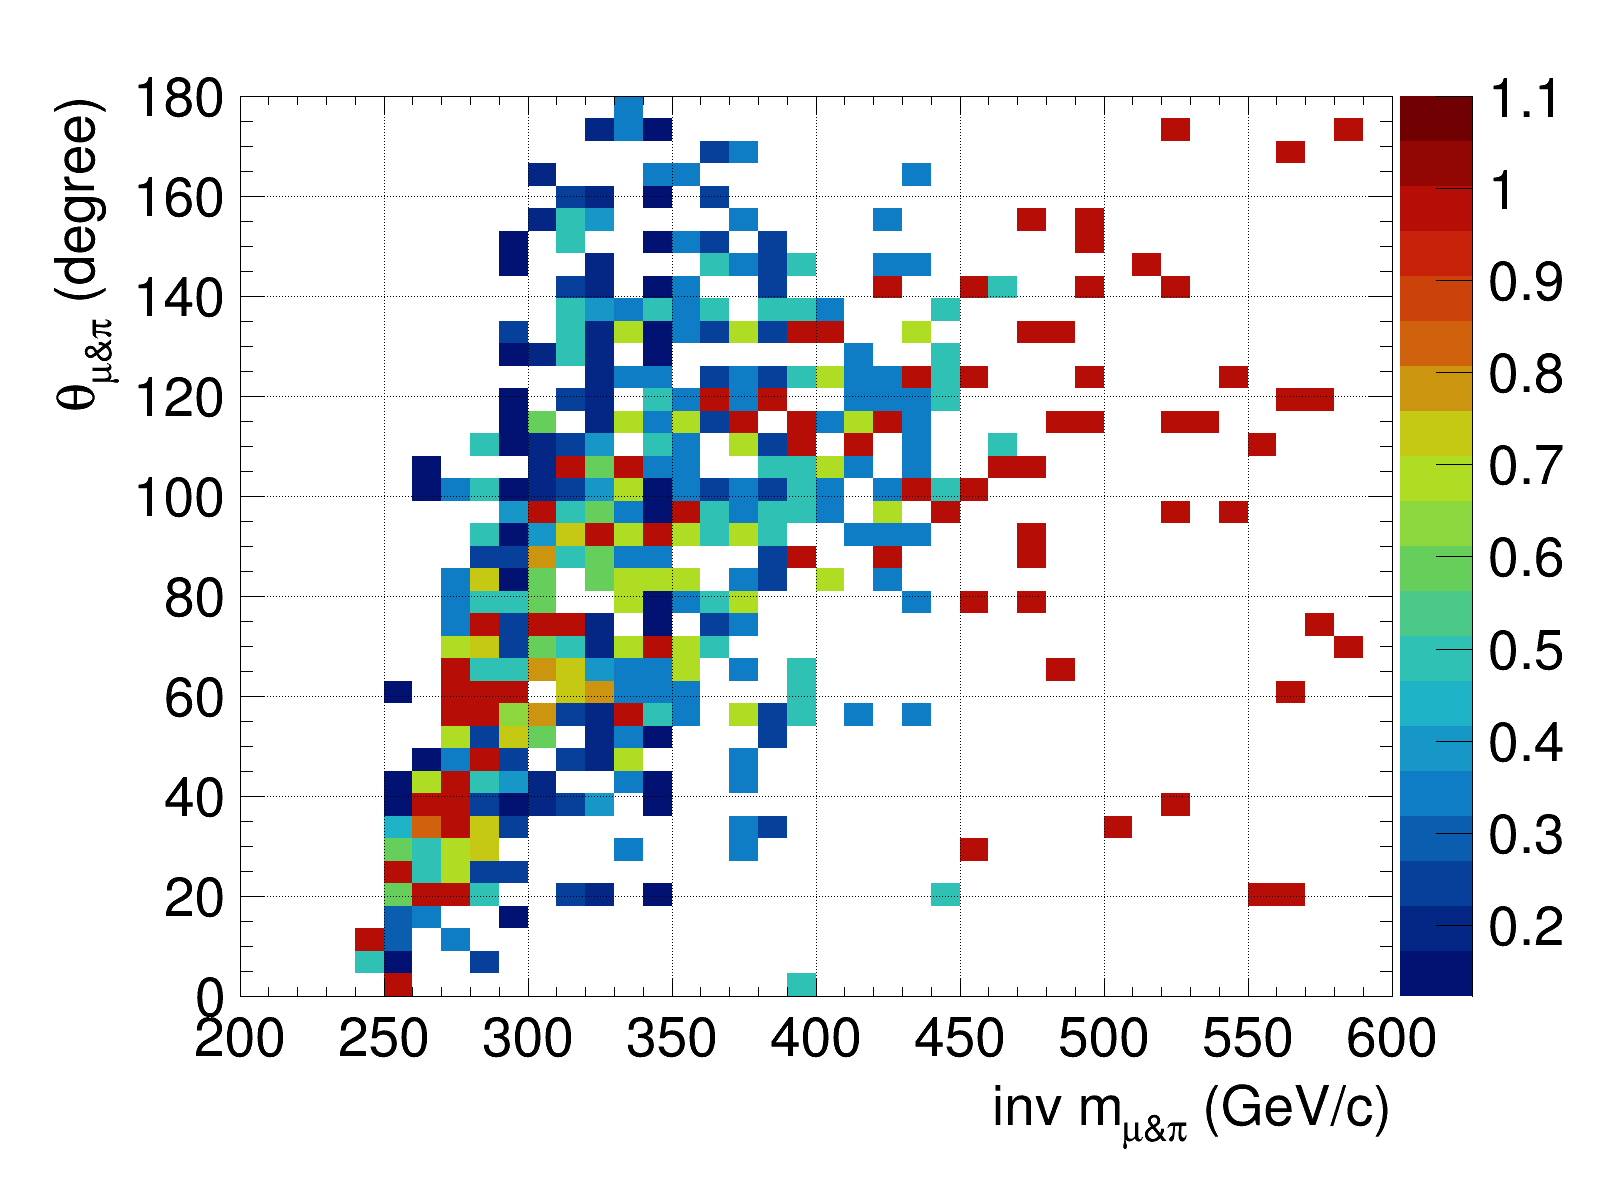
\includegraphics[width=\textwidth]{fig/hnl_sfgmu_mpinvm_colnor_vs_mpang_hist2d_al9_SM.png}
                \caption{SM $\nu$.}
                \label{fig:sm-mmupi}
           \end{subfigure}
           \caption{$\tmupi$ plotted against $\mmupi$.}
           \label{fig:mmupi-mupiang}
        \end{figure}

        \textbf{$\mu$-$\pi$ $\dpt$ cut} - Similar to the previous kinematic cuts, the net transverse momentum of $\mu$ and $\pi$ should be small while that for the SM event would have a much larger range as shown in Fig.~\ref{fig:mmupi-dpt}. By placing the cut, $\dptmupi<15~\mevc$, $8$ HNL events survived with $0$ SM backgrounds.
        
        \begin{figure}[!htb]
           \centering
           \begin{subfigure}{0.45\textwidth}
                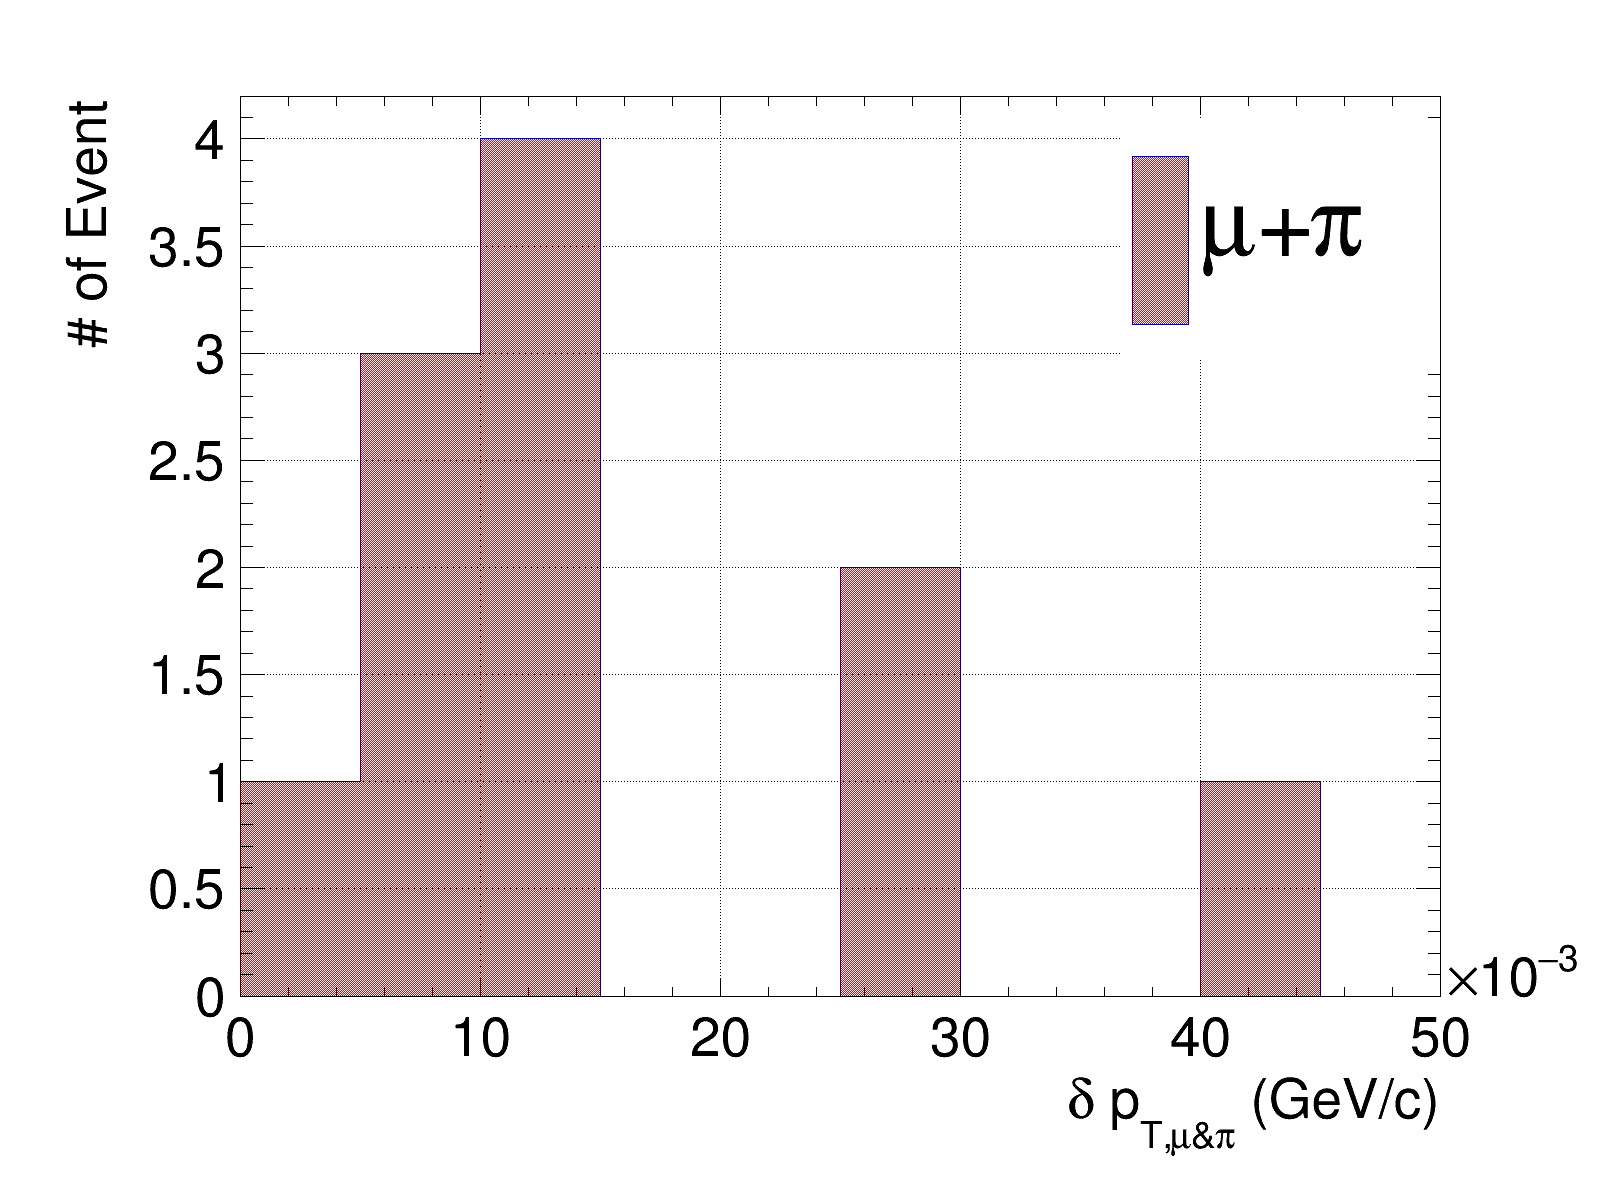
\includegraphics[width=\textwidth]{fig/hnl_sfgmu_mpdpt_stack_al9_300_aftmupikin.png}
                \caption{HNL.}
                \label{fig:hnl-mupidpt}
           \end{subfigure}
           \begin{subfigure}{0.45\textwidth}
                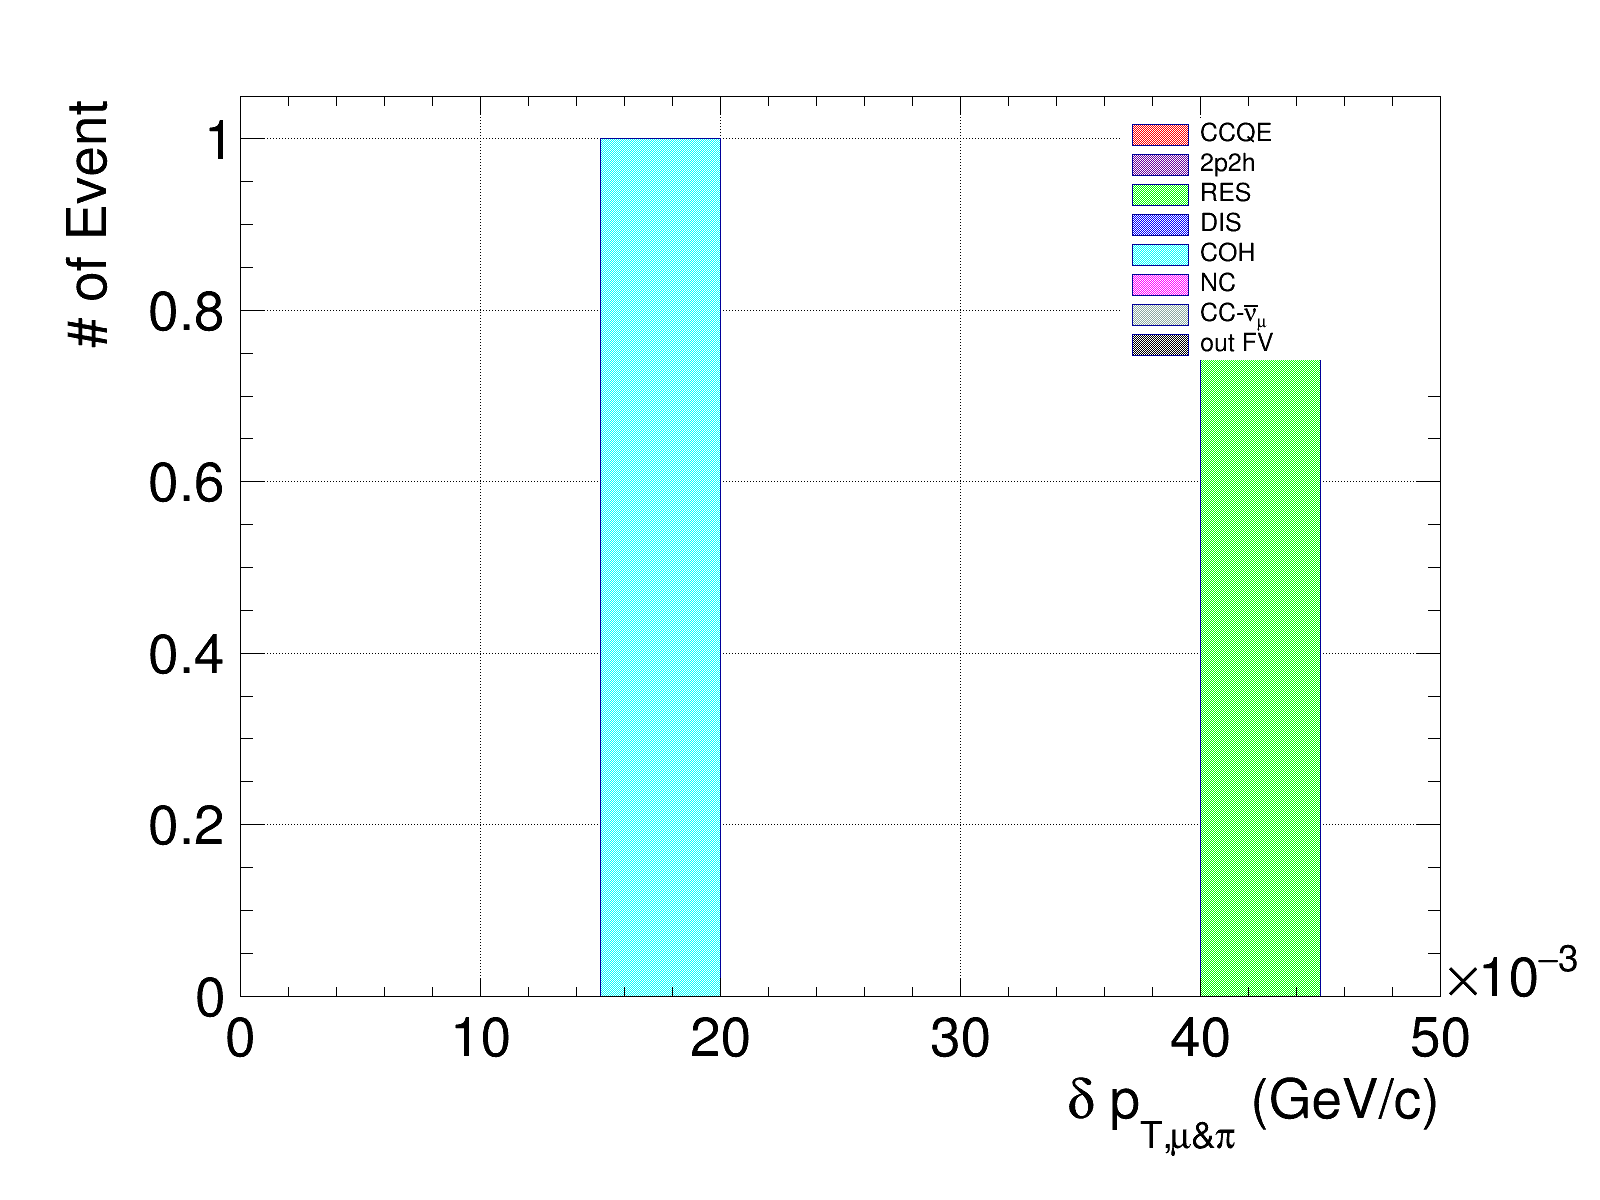
\includegraphics[width=\textwidth]{fig/hnl_sfgmu_mpdpt_stack_al9_SM_aftmupikin.png}
                \caption{SM $\nu$.}
                \label{fig:sm-mupidpt}
           \end{subfigure}
           \caption{$\dptmupi$ distributions for HNL and SM $\nv$.}
           \label{fig:mmupi-dpt}
        \end{figure}

    
    \subsubsection{Background estimation}
        A comprehensive background estimation is not finished yet, but it is suggesting, from Fig.~\ref{fig:sm-mupidpt}, and expected that coherent pion production is the dominant source. 
        From a crude estimation, as shown in Fig.~\ref{fig:coh-bkg}, the area under the fitted curve for $\dptmupi<15~\mevc$ is approximately $0.5$. 
        \begin{figure}[!htb] 
            \centering
            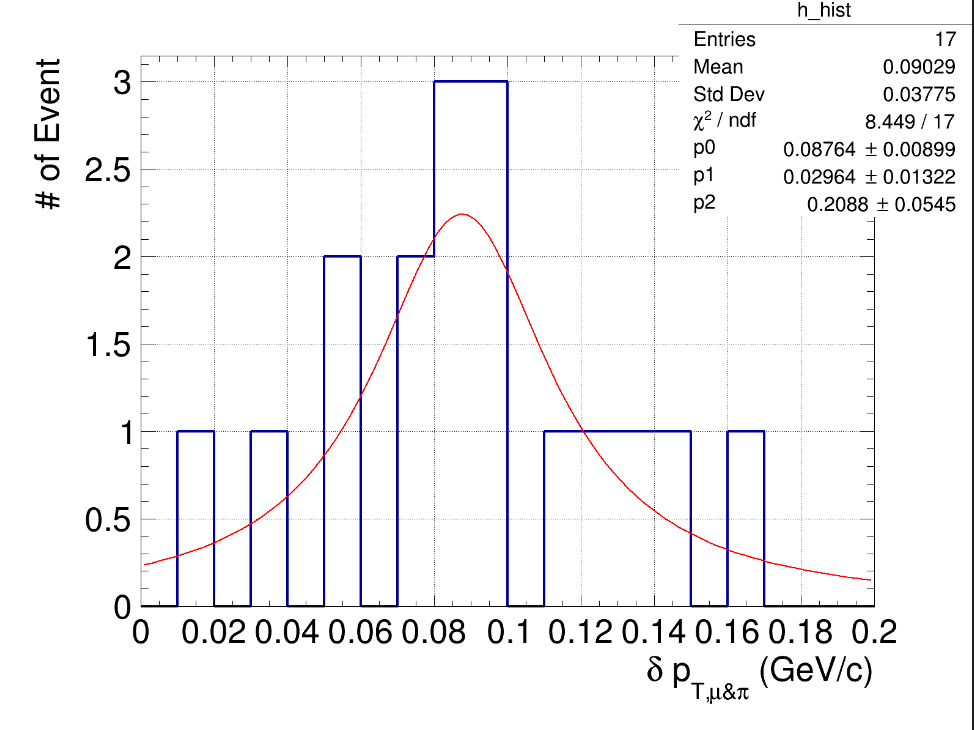
\includegraphics[width=0.5\linewidth]{fig/COH.png}
            \caption{Coherent background estimation.}
            \label{fig:coh-bkg}
        \end{figure}    
        
    \subsubsection{Sensitivity extraction}
        Sensitivity is extracted using the $CL_s$ method~\cite{Read_2002}.
        $CL_x$ is defined as $\textrm{Prob}(N\leq N_{\textrm{obs}}| \mu = x)$, i.e. the probability of predicting a number of events smaller or equal to the number of observed events assuming model $x$. When $x=b$ or $x=s+b$, it is the background-only model or the the signal plus background model.
        Then, $CL_s$ is defined as 
        \begin{equation}
            CL_s = \frac{CL_{s+b}}{CL_{b}} = \frac{\textrm{Prob}(N\leq N_{\textrm{obs}}| \mu = s+b)}{\textrm{Prob}(N\leq N_{\textrm{obs}}| \mu = b)} = \alpha,
        \end{equation}
        where $1-\alpha$ is the confidence level.

        For a target confidence level, $f$, one starts from $s=0$ and iterate with increasing $s$ to find the largest $s_{up}$ such that $\alpha < 1-f$. 
        Then $s_{up}$ is the upper limit for the number of signal events at confidence level $f$ such that the background-only model is not rejected. 
        When a more detailed background model is available, it is conventional to pick the median number of background events to evaluate $s_{up}$.
        A limit can then be placed on the mixing element $\umas$ from its proportional relation to $s_{up}$.

        Specifically in the above example, $100,000$ \genie events were simulated using \code{BeamHNL}. 
        The total number of protons on target (POT) required to produce these HNL events are calculated from \code{BeamHNL} output to be approximately $0.81\times10^{21}$ assuming $\umas=10^{-7}$. 
        Hence, we expect $8/0.81\approx9.9$ selected signals per $10^{21}$ POT.
        For this estimation, background is taken to be $0.5$, then $s_{up}$ is calculated to be $2.3$. 
        Hence, the limit on $\umas$ is calculated as 
        \begin{align}
            (\frac{U_{up}}{10^{-7}})^2 & =  2.3 / 9.9 \\
            U_{up} & = 10^{-7} \times \sqrt{2.3/89} = 4.8\times10^{-8}
        \end{align}

        \subsubsection{Discussion}
        This result is larger than the limit placed by the previous search, $U_{up}\approx4\times10^{-9}$, for $\mn=300~\mev$. 
        However, it is roughly of the same order of magnitude. 
        Moreover, the current result includes only events in SFGD, which is only about $1/3$ in volume compared to the vertical TPCs. 
        Most importantly, this preliminary result demonstrates that SFGD can also provide excellent signal-background separation for HNL searches.
        Hence, it will definitely improve the limits by adding it to the existing search. 
        Next step is to extend the selection to the whole upgraded ND280 when the HAT reconstruction becomes available and investigate the overall improvement in HNL sensitivity brought by the upgrade. 
 